\documentclass{article}
\usepackage[a4paper, portrait, margin=1.1811in]{geometry}
\usepackage[english]{babel}
\usepackage[utf8]{inputenc}
\usepackage[T1]{fontenc}
\usepackage{helvet}
\usepackage{etoolbox}
\usepackage{graphicx}
\usepackage{listings}
\usepackage{titlesec}
\usepackage{caption}
\usepackage{booktabs}
\usepackage{xcolor} 
\usepackage[colorlinks, citecolor=cyan]{hyperref}
\usepackage{caption}
\usepackage{tikz-qtree}
\usepackage{latexsym}
\usepackage{algorithm}
\usepackage{algpseudocode}
\captionsetup[figure]{name=Figure}
\graphicspath{ {./images/} }
\usepackage{scrextend}
\usepackage{fancyhdr}
\usepackage{graphicx}
\newcounter{lemma}
\newtheorem{lemma}{Lemma}
\newcounter{theorem}
\newtheorem{theorem}{Theorem}

\fancypagestyle{plain}{
	\fancyhf{}
	\renewcommand{\headrulewidth}{0pt}
	\renewcommand{\familydefault}{\sfdefault}
}

%\pagestyle{plain}
\makeatletter
\patchcmd{\@maketitle}{\LARGE \@title}{\fontsize{16}{19.2}\selectfont\@title}{}{}
\makeatother

\usepackage{authblk}
\renewcommand\Authfont{\fontsize{10}{10.8}\selectfont}
\renewcommand\Affilfont{\fontsize{10}{10.8}\selectfont}
\renewcommand*{\Authsep}{, }
\renewcommand*{\Authand}{, }
\renewcommand*{\Authands}{, }
\setlength{\affilsep}{2em}  
\newsavebox\affbox
\author{\textbf{Olteanu Fabian Cristian}}
\affil{FMI, AI Master, Year 1
}

\titlespacing\section{0pt}{12pt plus 4pt minus 2pt}{0pt plus 2pt minus 2pt}
\titlespacing\subsection{12pt}{12pt plus 4pt minus 2pt}{0pt plus 2pt minus 2pt}
\titlespacing\subsubsection{12pt}{12pt plus 4pt minus 2pt}{0pt plus 2pt minus 2pt}


\titleformat{\section}{\normalfont\fontsize{10}{15}\bfseries}{\thesection.}{1em}{}
\titleformat{\subsection}{\normalfont\fontsize{10}{15}\bfseries}{\thesubsection.}{1em}{}
\titleformat{\subsubsection}{\normalfont\fontsize{10}{15}\bfseries}{\thesubsubsection.}{1em}{}

\titleformat{\author}{\normalfont\fontsize{10}{15}\bfseries}{\thesection}{1em}{}

\title{\textbf{\huge Knowledge Representation and Reasoning Project 1}}
\date{}    

\begin{document}

\pagestyle{headings}	
\newpage
\setcounter{page}{1}
\renewcommand{\thepage}{\arabic{page}}


	
\captionsetup[figure]{labelfont={bf},labelformat={default},labelsep=period,name={Figure }}	\captionsetup[table]{labelfont={bf},labelformat={default},labelsep=period,name={Table }}
\setlength{\parskip}{0.2em}
	
\maketitle
	
\noindent\rule{15cm}{0.4pt}

\section{Resolution}
Let us consider the following knowledge base:


KB
$\left\{
\begin{tabular}{p{.8\textwidth}}
\begin{enumerate}
		\item Every DOTA2 player is a gamer.
		\item There are DOTA2 players who are professional.
		\item Some professional DOTA2 players who purchase Divine Rapier lose games.
		\item Anyone who loses games gets angry.
\end{enumerate}
\end{tabular}
\right.$

We want to prove that the following Question is logically entailed from our KB by applying the Resolution algorithm:

\centerline{5. Do some gamers who purchase Divine Rapier get angry?} 

\subsection{Representing the KB in FOL (a)}
The above written KB can be expressed in FOL in the following way:

KB
$\left\{
\begin{tabular}{p{.8\textwidth}}
\begin{enumerate}
		\item $\forall x. DOTA2\_Player(x) \supset Gamer(x)$
		\item $\exists x. DOTA2\_Player(x) \land Pro(x)$
		\item $\exists x. PRO(x) \land Buys\_Rapier(x)\land Loses\_Games(x)$
		\item $\forall x. Loses\_Games(x) \supset Gets\_Angry(x)$
		\item $\exists x. Gamer(x) \land Buys\_Rapier(x) \land Gets\_Angry(x)$.
\end{enumerate}
\end{tabular}
\right.$

For the sake of simplicity, we can write it in the following way: 

KB
$\left\{
\begin{tabular}{p{.8\textwidth}}
\begin{enumerate}
		\item $\forall x. P_1(x) \supset P_2(x)$
		\item $\exists x. P_1(x) \land P_3(x)$
		\item $\exists x. P_3(x) \land P_4(x)\land P_5(x)$
		\item $\forall x. P_5(x) \supset P_6(x)$
		\item $\exists x. P_2(x) \land P_4(x) \land P_6(x)$.
\end{enumerate}
\end{tabular}
\right.$

\subsection{Proving manually that the Question is logically entailed from the KB (b)}
In order to apply the resolution algorithm, we must first transform the KB written in FOL in the conjunctive normal form (CNF), after which the following transformation happens:

CNF
$\left\{
\begin{tabular}{p{.8\textwidth}}
\begin{enumerate}
		\item $\neg P_1(x) \lor P_2(x)$
		\item $P_1(V)$
		\item $P_3(V)$
		\item $P_4(V)$
		\item $P_5(V)$
		\item $\neg P_5(x) \lor P_6(x)$
		\item $P_2(V) \land P_4(V) \land P_6(V)$,
\end{enumerate}
\end{tabular}
\right.$

where V is a Skolem constant (we now have seven members in the list because we can "divide" into individual items logical sequences like number 2 from the last page: $P_1(x) \land P_3(x)$ becomes 2. $P_1(x)$ and 3. $P_3(x)$). 

Lastly, we need to prove that the negated form of the question that we want to prove is logically entailed from our KB is not satisfiable. After negating, our converted KB looks like this:

CNF
$\left\{
\begin{tabular}{p{.8\textwidth}}
\begin{enumerate}
		\item $\neg P_1(x) \lor P_2(x)$
		\item $P_1(V)$
		\item $P_3(V)$
		\item $P_4(V)$
		\item $P_5(V)$
		\item $\neg P_5(x) \lor P_6(x)$
		\item $\neg P_2(V) \lor \neg P_4(V) \lor \neg P_6(V)$.
\end{enumerate}
\end{tabular}
\right.$
\begin{center}
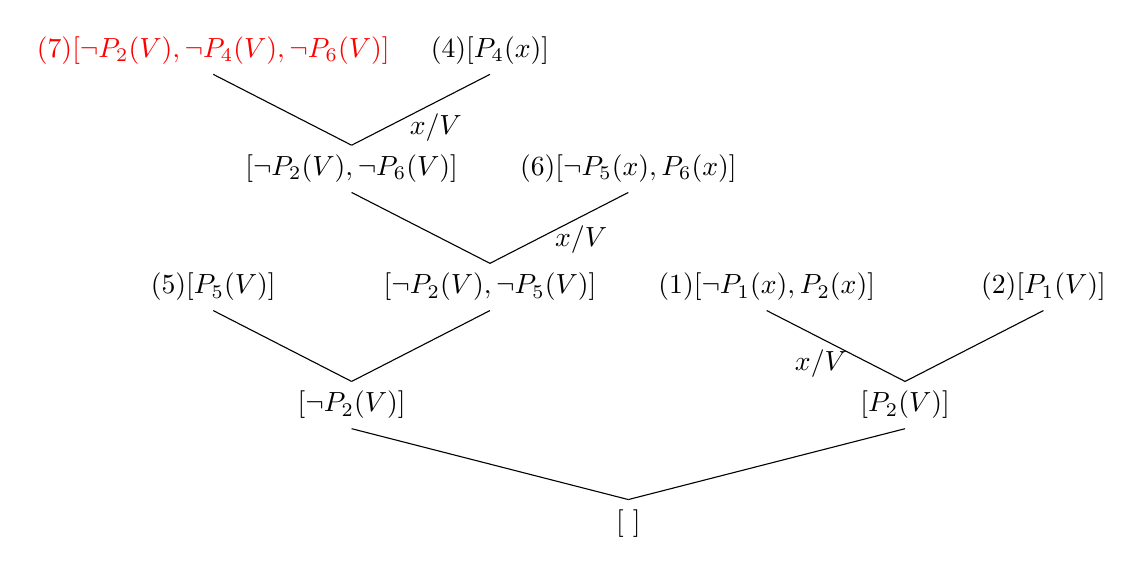
\begin{tikzpicture}[
  grow'=up,
  level 1/.style={sibling distance=20em},
  level 2/.style={sibling distance=10em}]
\node (f) {[ ]} 
child {
	node (-1) {$[\neg P_2(V)]$}
	child {node (0r) {(5)$[P_5(V)]$}}
child {
	node (0) {$[\neg P_2(V), \neg P_5(V)]$}
child { 
	node (1l) {$[\neg P_2(V),\neg P_6(V)]$}
		child {node (2ll) {\color{red}$(7)[\neg P_2(V),\neg P_4(V),\neg P_6(V)]$}}
		child {node (2lr) {$(4)[P_4(x)]$}}
}
child {
	node (1m) {(6)$[\neg P_5(x), P_6(x)]$}
}
}}
child {
	node (1r) {$[P_2(V)]$}
		child {node (2rl) {(1)$[\neg P_1(x),P_2(x)]$}}
		child {node (2rr) {(2)$[P_1(V)]$}}
};

   \begin{scope}[nodes = {draw = none}]
      \path (1l) -- (2lr) node [near start, right]  {$x/V$};
      \path (1r) -- (2rl) node [near start, left]  {$x/V$};
      \path (-1) -- (1m) node [near end, right]  {$x/V$};
   \end{scope}
\end{tikzpicture}
\end{center}

Thus, we have proven that the negated form of sentence 5 is unsatisfiable given our KB. In conclusion, the sentence: "Some gamers who purchase Divine Rapier get angry" is logically entailed from our KB. 

\subsection{Implementing the Resolution Algorithm in Prolog (c)}
	The Resolution algorithm can be expressed in the following way, using pseudocode \cite{Resolution}:
	
\algrenewcommand\algorithmicrequire{\textbf{Input:}}
\algrenewcommand\algorithmicensure{\textbf{Output:}}
\begin{algorithm}
\begin{algorithmic}
\caption{Res(S)}\label{alg:cap}
\Require $S$, a finite set of propositional clauses (of form [[w, s, n(p)], [a, n(w), r, t],[[q]])
\Ensure $S$ is satisfiable or unsatisfiable
\If{$[]\in S$}
	\State \Return unsat
\ElsIf {There are two clauses in $S$ such that they resolve to produce another clause not already in S}
	\State Add the new resolvent clause to S and remove the clauses used to obtain it
	\State Res(S)
	\Else \State \Return sat
\EndIf
\end{algorithmic}
\end{algorithm}

To implement this algorithm in Prolog, based on the pseudocode presented above, I followed this way of thinking:
\begin{itemize}
	\item The implemented algorithm returns false if the given set of clauses (KB) is satisfiable and true if it is unsatisfiable,
	\item For the resolution procedure I implemented a predicated called res/1 which takes KB as a parameter. The stop condition for the predicate is finding an empty list as a member.
	\item If there's no empty list in the KB, it does the following:
		\begin{enumerate}
			\item The KB is sorted using the built-in predicate sort/2\cite{sortpred} to remove tautologies,
			\item It takes a member clause from KB (Clause1) using the built-in predicate member/2\cite{memberpred},
			\item It takes a different member clause (Clause2) from KB,
			\item It selects a Subclause from Clause1, using the built-in predicate select/3\cite{selectpred},
			\item It checks if the negated Subclause is a member of Clause2; if it is, it selects the clauses from which the two subclauses originate and appends them to a Resolvent (using a built-in predicate called append/3\cite{appendpred}),
			\item The Resolvent is sorted (for the same effect as in step 1),
			\item The two clauses that generated the Resolvent are delete from the KB using a built in predicate delete/3\cite{deletepred},
			\item If the Resolvent is empty, return true (unsatisfiable),
			\item Otherwise, append the Resolvent to the new KB and continue recursively with the new KB.
		\end{enumerate}
\end{itemize}

For the sake of reading input from files, I also implemented a predicate called read\_clauses\_from\_file/2, which applies the res predicate to each line of input and outputs whether the clause set is satisfiable or unsatisfiable in the terminal.

To run the Prolog script on the set of clauses presented in the first page, it needs to be rewritten in the following way:
$$
KB=[[not(a), b], [a], [c], [d], [e], [not(e), f], [not(b), not(d), not(f)]].
$$
The letters a through f are direct mappings of the clauses $P_1$ through $P_6$ from page 2. Querying 
$$
KB=[[not(a), b], [a], [c], [d], [e], [not(e), f], [not(b), not(d), not(f)]], res(KB).
$$
yields the output "unsat", as expected.

\subsection{Running the Resolution Algorithm on Other Sets of Propositional Clauses (d)}
Implementing the read\_clauses\_from\_file/2 predicate and placing it inside of a main/0 predicate, along with creating a data.in file allows the Prolog script to swiftly compute the output for each of the following sets of clauses:
\begin{enumerate}
	\item $[[not(a), b], [c,d], [not(d), b], [not(b)], [not(c), b], [e], [a, b, not(f), f]]$ : \colorbox{red}{unsat}
	\item $[[not(b),a], [not(a),b,e], [a, not(e)], [not(a)], [e]]$ : \colorbox{red}{unsat}
	\item $[[not(a),b], [c,f], [not(c)], [not(f),b], [not(c),b]]$ : \colorbox{green} {sat}
	\item $[[a,b], [not(a), not(b)], [c]]$ : \colorbox{green}{sat}.
\end{enumerate} 

\section{Implementing the Davis-Putnam Procedure in Prolog}
Like the Resolution algorithm, the Davis-Putnam procedure also checks whether a finite set of clauses is satisfiable, but is generally faster. It also returns a list of truth values assigned to clauses from the Knowledge Base when it is satisfiable.

The algorithm, presented in pseudocode, is the following\cite{Resolution}: 
\begin{algorithm}
\begin{algorithmic}
\caption{DP(KB)}\label{alg:cap}
\Require $KB$, a finite set of propositional clauses (of form [[w, s, n(p)], [a, n(w), r, t],[[q]])
\Ensure are the clauses from $KB$ satisfiable or unsatisfiable, YES or NO?
\If{KB is empty}
	\State \Return YES
\EndIf
\If {KB contains []} \State \Return NO
\EndIf
\State p $\gets$ some atom from KB
\If {DP(KB $\cdot$ p)=YES}
\State \Return YES
\Else 
\State \Return DP(C $\cdot$ $\neg p$)
\EndIf
\end{algorithmic}
\end{algorithm}

The mathematical definition for the dot operation can be expressed as such:
$$
C \cdot m=\{c | c \in C, m \not\in c\} \cup \{(c- \neg m) | c \in C, m \not\in c, \neg m \in c\}.
$$

The operation can be computed using the following algorithm: For each L from C:
\begin{enumerate}
	\item if L contains m, remove L from C,
	\item if L contains $\neg m$, remove $\neg m$ from L.
\end{enumerate}

Another challenge in implementing the algorithm is finding optimal strategies of choosing p. Two of those that were used were
\begin{itemize}
	\item p appears in the shortest clause(s) in KB,
	\item p is the most balanced atom.
\end{itemize}

Taking all of these facts into account, the outline of the implementation of the algorithm was the following:
\begin{enumerate}
	\item A custom predicate called kb\_dot\_p/3 was implemented, which performs the dot operation. It is based on the two steps from above and uses two custom predicates called negate/2 and delete\_parameter/3 to perform the second step. The first step is achieved through the built-in findall/3\cite{findallpred} predicate which filters KB to exclude all clauses that include p. For the second step, the predicate delete\_parameter/3 uses maplist/3\cite{maplistpred} to filter the whole KB using the custom delete\_occurences\_of\_p/3 predicate (which filters only one clause from KB to remove ocurences of p).
	\item For the selection of p, two predicates were created corresponding to the two different strategies used. The first one is called select\_shortest\_p/2 (finds the list of minimum length, selects a member from that list and assigns it to P). The second one is select\_largest\_p/2, which does the opposite of the first selector. 
	\item There are two versions of the Davis-Putnam procedures implemented as two different predicates. The first one is dp\_shortest\_clauses\_p/2 and uses the select\_shortest\_p/2 predicate. Its implementation is very close to the pseudocode, the only addition being that of the truth values for the literals in a list. The second predicate is called dp\_largest\_clauses\_p/2 and apart from using the other selection predicate is exactly the same.
	\item Similar to the Resolution algorithm implementation, the prolog script in which the Davis-Putnam procedure was implemented also reads input from a file, but two different predicates had to be implemented evaluate the two custom predicates on the clause sets 
	
	(read\_clauses\_from\_file1/2 and read\_clauses\_from\_file2/2).
\end{enumerate}

The following input was used with the script:
\begin{enumerate}
	\item $[[toddler],[not(toddler),child],[not(child),not(male),boy],[not(infant),child],$ \hfill \\ $[not(child),not(female),girl], [female], [girl]]$
	\item $[[toddler],[not(toddler),child],[not(child),not(male),boy],[not(infant),child],$ \hfill \\$ [not(child),not(female),girl], [female], [not(girl)]]$
	\item $[[not(a),b],[c,d],[not(d),b],[not(c),b],[not(b)],[e],[a,b,not(f),f]]$
	\item $[[not(b),a],[not(a),b,e],[e],[a, not(e)],[not(a)]]$
	\item $[[not(a),not(e),b],[not(d),e,not(b)],[not(e),f,not(b)],[f,not(a),e],[e,f,not(b)]]$
	\item $[[a,b],[not(a),not(b)] ,[not(a),b] ,[a,not(b)]]$
\end{enumerate}

After running the D-P predicates on the input, the following output resulted:

\begin{verbatim}
--------Strategy 1: P appears in the shortest clauses--------------
[toddler/true,child/true,female/true,girl/true,not(male)/true]
NO
NO
NO
[not(a)/true,not(d)/true,not(e)/true,f/true]
NO
------------Strategy 2: P is in the largest clauses-----------------
[not(male)/true,girl/true,child/true,toddler/true,female/true]
NO
NO
NO
[not(a)/true,not(d)/true,not(e)/true,f/true]
NO
-------------------------------------------------------------------
\end{verbatim}

After also running the Resolution script on the same input, it also assigned the same sat/unsat values to each set of clauses, confirming the correctness of the results.

\newpage
\bibliographystyle{IEEEtran}
\begin{thebibliography}{1.7} 
	\bibitem[1]{Resolution} \color{cyan}Ronald Brachman, Hector Levesque, “Knowledge Representation and Reasoning,” \textit{Morgan Kaufmann}, p. 54-78, 2004
	\bibitem[2]{sortpred} \url{https://www.swi-prolog.org/pldoc/man?predicate=sort/2}
	\bibitem[3]{memberpred} \url{https://www.swi-prolog.org/pldoc/doc_for?object=member/2}
	\bibitem[4]{selectpred} \url{https://www.swi-prolog.org/pldoc/doc_for?object=select/3}
	\bibitem[5]{appendpred} \url{https://www.swi-prolog.org/pldoc/doc_for?object=append/3}
	\bibitem[6]{deletepred} \url{https://www.swi-prolog.org/pldoc/doc_for?object=delete/3}
	\bibitem[7]{findallpred} \url{https://www.swi-prolog.org/pldoc/man?predicate=findall/3}
	\bibitem[8]{maplistpred} \url{https://www.swi-prolog.org/pldoc/doc_for?object=maplist/3}
\end{thebibliography}

\newpage

% --- ugly internals for language definition ---
%
\makeatletter

% initialisation of user macros
\newcommand\PrologPredicateStyle{}
\newcommand\PrologVarStyle{}
\newcommand\PrologAnonymVarStyle{}
\newcommand\PrologAtomStyle{}
\newcommand\PrologOtherStyle{}
\newcommand\PrologCommentStyle{}

% useful switches (to keep track of context)
\newif\ifpredicate@prolog@
\newif\ifwithinparens@prolog@

% save definition of underscore for test
\lst@SaveOutputDef{`_}\underscore@prolog

% local variables
\newcount\currentchar@prolog

\newcommand\@testChar@prolog%
{%
  % if we're in processing mode...
  \ifnum\lst@mode=\lst@Pmode%
    \detectTypeAndHighlight@prolog%
  \else
    % ... or within parentheses
    \ifwithinparens@prolog@%
      \detectTypeAndHighlight@prolog%
    \fi
  \fi
  % Some housekeeping...
  \global\predicate@prolog@false%
}

% helper macros
\newcommand\detectTypeAndHighlight@prolog
{%
  % First, assume that we have an atom.
  \def\lst@thestyle{\PrologAtomStyle}%
  % Test whether we have a predicate and modify the style accordingly.
  \ifpredicate@prolog@%
    \def\lst@thestyle{\PrologPredicateStyle}%
  \else
    % Test whether we have a predicate and modify the style accordingly.
    \expandafter\splitfirstchar@prolog\expandafter{\the\lst@token}%
    % Check whether the identifier starts by an underscore.
    \expandafter\ifx\@testChar@prolog\underscore@prolog%
      % Check whether the identifier is '_' (anonymous variable)
      \ifnum\lst@length=1%
        \let\lst@thestyle\PrologAnonymVarStyle%
      \else
        \let\lst@thestyle\PrologVarStyle%
      \fi
    \else
      % Check whether the identifier starts by a capital letter.
      \currentchar@prolog=65
      \loop
        \expandafter\ifnum\expandafter`\@testChar@prolog=\currentchar@prolog%
          \let\lst@thestyle\PrologVarStyle%
          \let\iterate\relax
        \fi
        \advance \currentchar@prolog by 1
        \unless\ifnum\currentchar@prolog>90
      \repeat
    \fi
  \fi
}
\newcommand\splitfirstchar@prolog{}
\def\splitfirstchar@prolog#1{\@splitfirstchar@prolog#1\relax}
\newcommand\@splitfirstchar@prolog{}
\def\@splitfirstchar@prolog#1#2\relax{\def\@testChar@prolog{#1}}

% helper macro for () delimiters
\def\beginlstdelim#1#2%
{%
  \def\endlstdelim{\PrologOtherStyle #2\egroup}%
  {\PrologOtherStyle #1}%
  \global\predicate@prolog@false%
  \withinparens@prolog@true%
  \bgroup\aftergroup\endlstdelim%
}

% language name
\newcommand\lang@prolog{Prolog-pretty}
% ``normalised'' language name
\expandafter\lst@NormedDef\expandafter\normlang@prolog%
  \expandafter{\lang@prolog}

% language definition
\expandafter\expandafter\expandafter\lstdefinelanguage\expandafter%
{\lang@prolog}
{%
  language            = Prolog,
  keywords            = {},      % reset all preset keywords
  showstringspaces    = false,
  alsoletter          = (,
  alsoother           = @$,
  moredelim           = **[is][\beginlstdelim{(}{)}]{(}{)},
  MoreSelectCharTable =
    \lst@DefSaveDef{`(}\opparen@prolog{\global\predicate@prolog@true\opparen@prolog},
}

% Hooking into listings to test each ``identifier''
\newcommand\@ddedToOutput@prolog\relax
\lst@AddToHook{Output}{\@ddedToOutput@prolog}

\lst@AddToHook{PreInit}
{%
  \ifx\lst@language\normlang@prolog%
    \let\@ddedToOutput@prolog\@testChar@prolog%
  \fi
}

\lst@AddToHook{DeInit}{\renewcommand\@ddedToOutput@prolog{}}

\makeatother
%
% --- end of ugly internals ---


% --- definition of a custom style similar to that of Pygments ---
% custom colors
\definecolor{PrologPredicate}{RGB}{000,031,255}
\definecolor{PrologVar}      {RGB}{024,021,125}
\definecolor{PrologAnonymVar}{RGB}{000,127,000}
\definecolor{PrologAtom}     {RGB}{186,032,032}
\definecolor{PrologComment}  {RGB}{063,128,127}
\definecolor{PrologOther}    {RGB}{000,000,000}

% redefinition of user macros for Prolog style
\renewcommand\PrologPredicateStyle{\color{PrologPredicate}}
\renewcommand\PrologVarStyle{\color{PrologVar}}
\renewcommand\PrologAnonymVarStyle{\color{PrologAnonymVar}}
\renewcommand\PrologAtomStyle{\color{PrologAtom}}
\renewcommand\PrologCommentStyle{\itshape\color{PrologComment}}
\renewcommand\PrologOtherStyle{\color{PrologOther}}

% custom style definition 
\lstdefinestyle{Prolog-pygsty}
{
  language     = Prolog-pretty,
  upquote      = true,
  stringstyle  = \PrologAtomStyle,
  commentstyle = \PrologCommentStyle,
  literate     =
    {:-}{{\PrologOtherStyle :-}}2
    {,}{{\PrologOtherStyle ,}}1
    {.}{{\PrologOtherStyle .}}1
}

% global settings
\lstset
{
  captionpos = below,
  frame      = single,
  columns    = fullflexible,
  basicstyle = \ttfamily,
}







\lstinputlisting[style=Prolog-pygsty, caption={Resolution Implementation in Prolog}]{resolution.pro}
\newpage
\lstinputlisting[style=Prolog-pygsty, caption={Davis-Putnam Procedure Implementation in Prolog}]{davis_putnam.pro}

\end{document}